\chapter{Processi di supporto}
\section{Documentazione}\label{s:documentazione}

\subsection{Scopo}

Scopo del processo di documentazione è la raccolta di tutto quanto sia utile per rendere consistente, coeso e ripetibile il processo di produzione.

\subsection{Ciclo di vita dei documenti}

Ogni documento segue le fasi seguenti nel suo ciclo di vita. Inoltre queste fasi si ripeteranno per tutto il tempo in cui anche il prodotto software sarà vivo.

Questo ciclo di vita sarà incrementale e tracciato dalle versioni.

Prodotto software e documentazione coesistono per consentire il raggiungimento dello scopo di questo processo.

\paragraph{Approvazione delle modifiche} A risultato delle riunioni interne il responsabile approva le modifiche e quindi anche le aggiunte che dovranno essere eseguite al documento in oggetto.

\paragraph{Redazione} Un documento viene redatto da uno o più redattori. Il documento durante la redazione verrà incrementato di tutto quanto deciso durante le riunioni. Il documento viene considerato redatto quando se ne è completata la stesura.

\paragraph{Verifica} Quando un documento è stato redatto viene verificato dalla figura del \textit{verificatore}, questo ne controllerà consistenza, validità e ortografia.

\paragraph{Approvazione e Rilascio} Quando il documento sarà stato verificato il responsabile approverà e rilascerà il documento seguendo le regole di versionamento definite.

\subsubsection{Ciclo di vita dei verbali}

I verbali seguono lo stesso ciclo di vita dei docuementi, ma non avranno fasi di ripetizione, in quanto verranno redatti, verificati e rilasciati solamente una volta. Un verbale non sarà infatti un documento modificabile.

\subsubsection{Ciclo di vita della documentazione sviluppatori microservizio WebApp}

La documentazione per gli sviluppatori riguardante il microservizio della WebApp segue lo stesso ciclo di vita dei documenti, senza però fasi di ripetizione, in quanto verrà redatta, verificata e rilasciata una volta sola dopo che la WebApp sarà stata terminata e approvata.

\subsection{Classificazione dei documenti}

I documenti vengono raggruppati in due classi principali definite dallo scopo delle stesse.

\subsubsection{Documenti ad uso interno}

I documenti ad uso interno sono destinati solo all'uso da parte dei membri del gruppo 

\begin{itemize}
    \item Verbali interni;
    \item Norme di progetto.
\end{itemize}

\subsubsection{Documenti ad uso esterno}

\begin{itemize}
    \item Verbali esterni;
    \item Analisi dei requisiti;
    \item Piano di progetto;
    \item Piano di qualifica;
    \item Documentazione per lo sviluppatore microservizio WebApp.
\end{itemize}

\subsection{Nome dei file codificato}

Tutti i documenti seguono le regole generali nella definizione del nome del file. Su queste regole possono esserci poi specifiche espansioni o eccezioni.

\subsubsection{Regole generali}
\paragraph{Notazione}I nomi dei file seguono la notazione \textit{Kebab case}.

\[[\text{titolo-del-documento}]\]

\paragraph{Per il VCS} Per consentire il funzionamento delle pipeline di verifica\footnote{Vedasi sezione \ref{s:verifica}} dei documenti, nel sistema di \textit{VCS} i documenti in tex vanno nominati come segue.

\[\text{d}\_[\text{titolo-del-documento}]\]

\subsubsection{Regole specifiche per i verbali}
I nomi file dei verbali vengono codificati secondo la seguente struttura:

\[[TTT]\_[AAMMGG]\_[N]\]

Con:
\begin{itemize}
    \item \textbf{TTT}: tipologia di verbale come da tabella \Ref{table:t_verbali} ;
    \item \textbf{AAMMGG}: data di svolgimento dell'incontro a cui fa riferimento il verbale con ordinazione anno mese giorno;
    \item \textbf{N}: numero del verbale con partenza da 1 da inserire nel caso siano stati fatti più incontri nella medesima giornata.
\end{itemize}

\begin{table}[h]
    \centering
    \begin{tabularx}{0.7\linewidth}{X | l}
        \textbf{Tipologia verbale} & \textbf{Prefisso}\\
        \hline
        Verbale interno & VIN \\
        Verbali esterni & VEX\\
        Verbali di sprint & SPR \\
    \end{tabularx}
    \caption{Tipologie verbali}
    \label{table:t_verbali}
\end{table}



\subsection{Sigle e abbreviazioni}

All'interno dei documenti per brevità e semplicità di lettura verranno spesso utilizzate sigle e abbreviazioni, di seguito quelle con porrtata generale.

\begin{center}
    \begin{tabularx}{\linewidth}{l | X }            
        \textbf{Sigla} & \textbf{Definizione}\\
        \hline
        \textbf{AdR} & Analisi dei requisiti\\
        \textbf{NdP}& Norme di progetto\\
        \textbf{PdP}& Piano di progetto\\
        \textbf{PdQ}& Piano di qualifica\\
        \textbf{MU}& Manuale Utente\\
        \textbf{MM}& Manauele Manutentore\\
    \end{tabularx}
\end{center}

\subsection{Struttura}

Ogni documento ufficiale prodotto deve seguire una struttura precisa e definita per garantire consistenza comunicativa. Su queste regole possono esserci poi specifiche espansioni o eccezioni.

\subsubsection{Regole generali}

La struttura per i documenti generali è la seguente:

\begin{center}
    \begin{tabularx}{\linewidth}{l | X }            
        \textbf{Sezione} & \textbf{Scopo}\\
        \hline
        Frontespizio/copertina & Definisce per il lettore le informazioni base sul documento e su chi lo ha redatto\\
        Registro delle modifiche & Sono presenti tutti i cambiamenti al documento\\
        Tavola dei contenuti & Contiene l'indice dei contenuti presenti nel documento \\
        Corpo del documento & Sono presenti tutte le informazioni comunicative del documento\\
    \end{tabularx}
\end{center}

\paragraph{Frontespizio/copertina} Nella copertina devono essere presenti:
\begin{itemize}
    \item il logo dell'Università di Padova in alto a sinistra;
    \item il logo del gruppo in alto a destra;
    \item nome del corso, anno accademico, titolo del documento e versione al centro;
    \item uso e destinatario, in forma tabellare, al centro.
\end{itemize}
Una versione già strutturata del frontespizio è presente nel repository \textit{global-assets}\footnote{\href{https://github.com/SWEasabi/global-assets}{https://github.com/SWEasabi/global-assets}}

\paragraph{Registro delle modifiche} Nella registro delle modifiche saranno presenti, in forma tabellare
\begin{itemize}
    \item versione;
    \item data;
    \item modifica;
    \item persone, in formato \textit{Cognome Nome}.
\end{itemize}

\paragraph{Tavola dei contenuti} La tavola dei contenuti viene generata automaticamente utilizzando \LaTeX.

\paragraph{Glossario} Nel glossario sono presenti tutti i termini specifici attinenti al documento. Tipograficamente sono definiti utilizzando dei paragrafi.

\paragraph{Corpo del documento} In questa sezione viene redatto utilizzando i capitoli il contenuto del documento.

\subsubsection{Regole specifiche per i verbali}

La struttura per i verbali è la seguente:

\begin{center}
    \begin{tabularx}{\linewidth}{l | X }            
        \textbf{Sezione} & \textbf{Scopo}\\
        \hline
        Frontespizio/copertina & Definisce per il lettore le informazioni base sul documento e su chi lo ha redatto\\
        Adempimenti burocratici & Definisce le informazioni generali del verbale\\
        Corpo del documento & Sono presenti tutte le informazioni comunicative del documento\\
    \end{tabularx}
\end{center}

\paragraph{Adempimenti burocratici}\footnote{In alcuni verbali legacy viene descritto come \textbf{Informazioni generali}} In questa sezione sono scritte in elenco puntato:

\begin{itemize}
    \item luogo e data dell'incontro:
	\begin{itemize}
		\item luogo;
		\item data;
	\end{itemize}
	\item presenze.
\end{itemize}

Nel corpo del documento devono essere presenti:

\begin{itemize}
    \item ordine del giorno;
    \item svolgimento;
    \item risultati.
\end{itemize}


\subsection{Stili testuali}
\subsection{Elementi grafici}
\subsection{Strumenti di redazione e tecnologici}

\paragraph{\LaTeX} Utilizzato per stendere i documenti principali poiché consente di utilizzare metodologie strutturate di versionamento\footnote{Vedasi sottosezione \Ref{sss:vcs} per ulteriori informazioni.} e di verifica dei contenuti redatti.

\paragraph{GitHub Actions} Per controllare la consistenza del documento è presente un'azione che controlla la compilazione del documento in \LaTeX.

\subsection{Workflows}

\subsubsection{Aggiunta a backlog}

Ogni issue e pull request aperte in submodules che fanno uso di questo workflow vengono aggiunte al GitHub Project dell'organizzazione.

\lstinputlisting{\gassets global-assets/yml/backlog.yml}

\subsubsection{Compilazione dei documenti, GitHub Page e Release}

\paragraph{Impostazione variabili d'ambiente} Per semplificare l'installazione del workflow nei diversi submodules dedicati alla documentazione è stato pensato un template che richiede modifiche solo nella sezione dedicata alla dichiarazione delle variabili d'ambiente. Queste variabili determinano come si chiameranno gli artifacts che produrrà il workflow (\texttt{REPO\_NAME}) e il titolo che verrà mostrato nella GitHub Page (\texttt{DISPLAY\_NAME}).

\lstinputlisting[linerange={1-5}]{\gassets global-assets/yml/compile_check.yml}

\textbf{Esempio per il documento corrente}\\

\begin{lstlisting}
on: [push, pull_request]

env:
  REPO_NAME: norme-di-progetto
  DISPLAY_NAME: Norme di progetto
\end{lstlisting}

\paragraph{Compilazione dei documenti} La compilazione avviene mediante \texttt{latexmk -lualatex} di tutti i file \texttt{.tex} che presentano nel nome il prefisso "d\_". Prima della compilazione il workflow si occupa anche di prelevare tutti i documenti presenti nei sottomoduli. Infine, dopo la compilazione, genera un artifact contenente esclusivamente i file in formato \texttt{.pdf} che saranno utilizzati nei prossimi job.

\lstinputlisting[linerange={7-31}]{\gassets global-assets/yml/compile_check.yml}

\paragraph{Creazione GitHub Page} Questa sezione si occupa di generare le pagine HTML che GitHub interpreterà e renderà disponibili. Il workflow fa uso della Action "apindex" per generare le pagine a partire da un template messo a disposizione nel sottomodulo global-assets.

\lstinputlisting[linerange={33-72}]{\gassets global-assets/yml/compile_check.yml}

\paragraph{Distribuzione GitHub Page} L'Action di GitHub dedicata al deploy consente la costruzione del sito web a partire dalle pagine HTML presenti nell'artifact generato nel job precedente. L'aggiornamento del sito web avviene esclusivamente al rilevamento di un tag (ad esempio il push della v1.0.0).


\lstinputlisting[linerange={74-101}]{\gassets global-assets/yml/compile_check.yml}

\paragraph{Nota} Per consentire a GitHub di rendere disponibile il sito web è necessario modificare un'impostazione del repository. Verificare, quindi, che in \texttt{Settings\rightarrow Pages\rightarrow Build and deployment} sia selezionata "GitHub Actions" come Source.

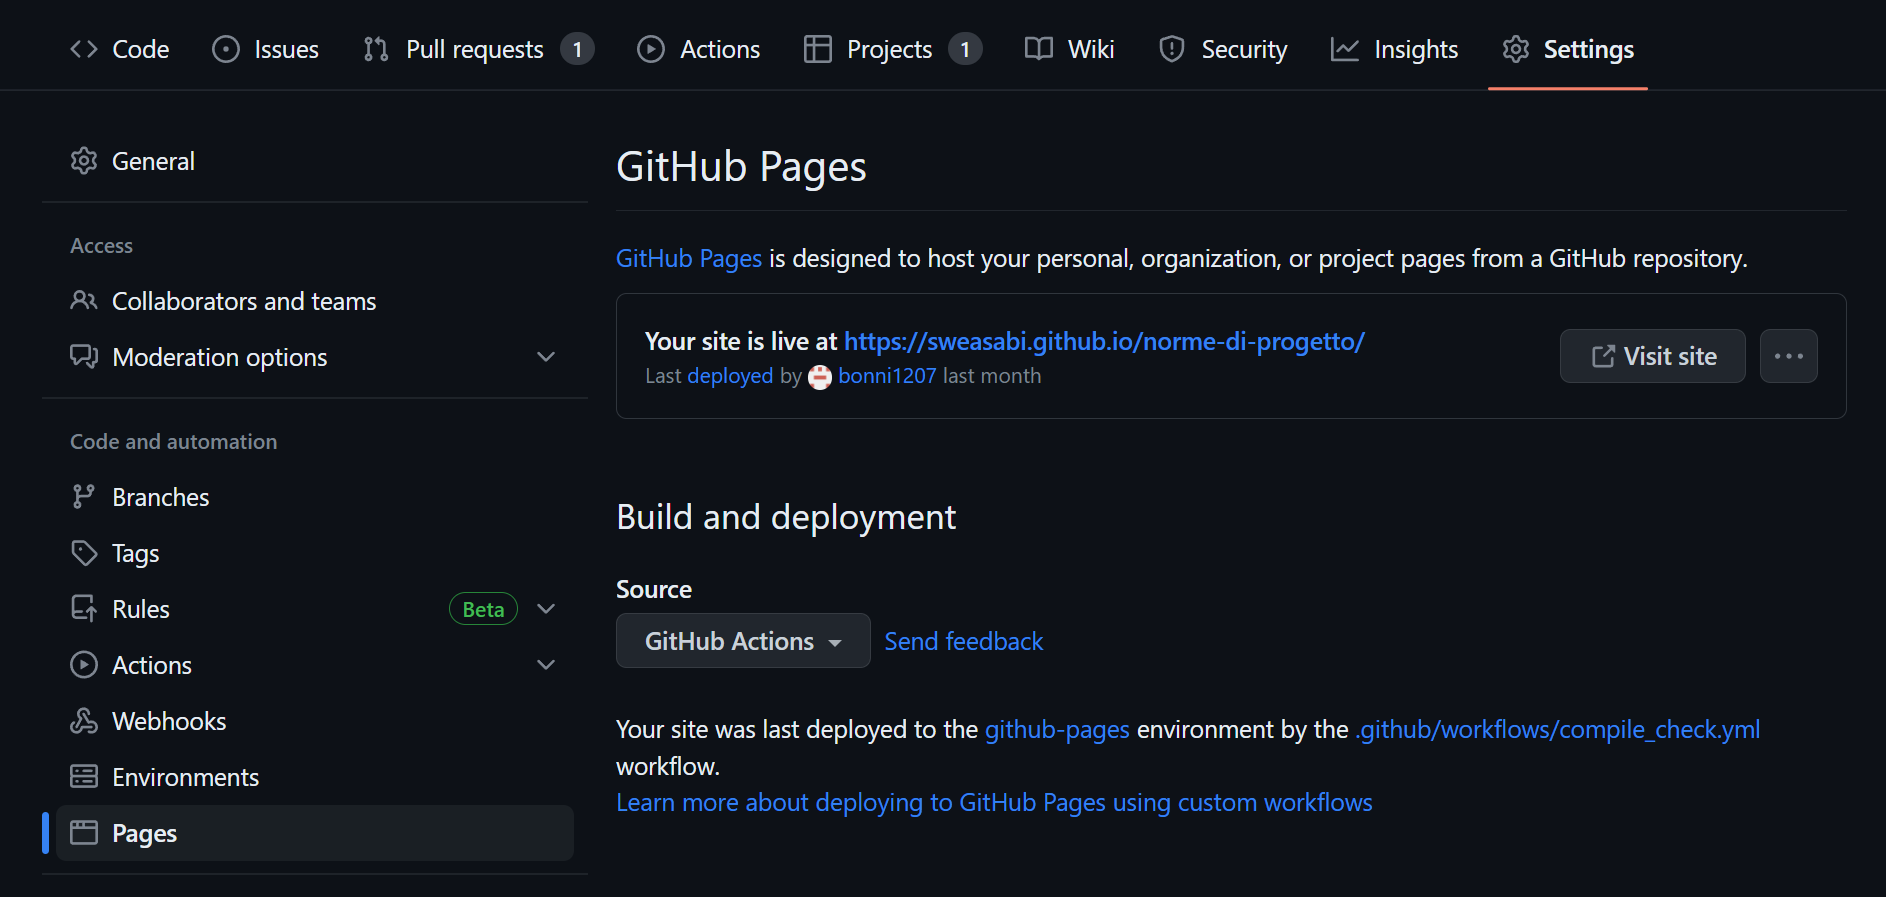
\includegraphics[width=\linewidth]{img/pages_actions.png}

\paragraph{Rilascio versione} Nell'ultima sezione i file in formato \texttt{.pdf} e privi di prefisso "d\_" vengono raccolti in un archivio \texttt{.zip} che viene allegato alla Release del repository. Il rilascio dell'archivio avviene esclusivamente al rilevamento di un tag (ad esempio il push della v1.0.0).

\lstinputlisting[linerange={103-124}]{\gassets global-assets/yml/compile_check.yml}

\section{Gestione di configurazione}\label{s:configurazione}

Per la configurazione del prodotto e per la gestione documentale vengono utilizzate varie strategie per organizzare e rendere consistente.

\subsection{Strumenti tecnologici}

\subsubsection{VCS}\label{sss:vcs} Per il versionamento e tracciamento delle modifiche apportate ai documenti e al codice steso durante il progetto viene utilizzato il \textit{version control system} Git. 

In abbinata a Git viene utilizzato GitHub per permettere facile collaborazione oltre ad accorpare in un unico luogo anche gli strumenti di ITS e CI/CD pipeline.

\subsubsection{ITS} Per il tracciamento delle issue viene utilizzato GitHub.

\subsection{Strutturazione dei repository}


\section{Gestione della qualità}\label{s:qualità}
\subsection{Scopo}
Scopo del processo di Gestione della qualità è di stabilire metriche precise per tutte le attività nell’ambito della verifica e della validazione.

In tal modo è possibile garantire il rispetto del livello
di qualità fissato.

Per approfondire le metriche utilizzate si rimanda al \textbf{PdQ}

\section{Gestione della verifica}\label{s:verifica}
\subsection{Scopo}

Scopo del processo di gestione della verifica è individuare errori all'interno del prodotto durante la sua produzione e la sua manutenzione.

Sia la documentazione\footnote{Vedasi sezione \ref{s:documentazione} per approfondire.} che il software sono soggetti a questo processo.


\section{Validazione}\label{s:validazione}

\subsection{Scopo} Scopo del processo di validazione è garantire che il prodotto sia conforme alle aspettative. La validazione garantisce che le linee guida delle \textbf{NdP} vengano rispettate.
